\documentclass[10pt,twocolumn]{article}

\usepackage[margin=0.75in]{geometry}
\usepackage{times}
\usepackage{microtype}
\usepackage{amsmath, amssymb}
\usepackage{graphicx}
\usepackage{booktabs}
\usepackage{enumitem}
\usepackage{float}
\usepackage{url}
\usepackage[hidelinks]{hyperref}
\usepackage[capitalise]{cleveref}

\title{\textbf{Native Animation Flow Matching: \\
Generating Stylized Animation from a Single Keyframe}}

\author{
Aaditya Baranwal, Grace Lim, Priyank Pathak, Xin Liang, Dawn Martin}
\date{}

\begin{document}
\maketitle

\begin{abstract}
We present \emph{Native Animation Flow Matching} (Native FM), a framework for generating short stylized-animation continuations conditioned on a single keyframe. Off-the-shelf video diffusion and Flow Matching models inherit a strong photorealism prior from their training data, and they reliably collapse the smears, impact frames, and morphing motions that define native animation. We refer to this failure as the \emph{realism trap}, and we address it on two fronts. First, we curate a Sakugabooru corpus of $11{,}869$ clips covering more than $240$ anime series and expand it into approximately $3.6$M keyframe-to-continuation pairs through a reproducible windowing pipeline. Second, we extend a Wan-based Flow Matching backbone with three coordinated modifications: a keyframe-preserving scheduler shift, a motion-aware per-frame loss reweighting, and a latent temporal-difference consistency regularizer. On a four-axis evaluation that combines continuation fidelity (CFS), temporal consistency (TCS), worst-segment quality (WorstSeg), and a diffusion-failure score (DFS), the 5B configuration of Native FM raises the FinalScore from $0.50$ to $0.65$. The improvement is concentrated in collapse-related axes: a $0.20$ reduction in DFS and a $0.09$ gain in WorstSeg, rather than raw fidelity. The relative training-loss reduction of $14.9\%$ over a single epoch is consistent with what FLUX- and Stable-Diffusion-style proxies achieve on their simpler velocity-MSE objective, despite the strictly harder composite loss optimized by Native FM.
\end{abstract}

\section{Introduction}

Modern video generation systems~\cite{ho2022video, blattmann2023stable, wan2025team} produce visually striking photorealism, yet they consistently fail on \emph{native animation}, the deliberately exaggerated and physics-violating motion that defines high-quality 2D animation. Trained on web-scale real-world video, these models inherit a strong realism prior in which gravity, inertia, and uniform lighting are baked in. The smears, impact frames, and squash-and-stretch deformations that drive expressive animation are smoothed away as a result. We refer to this failure mode as the \emph{realism trap}, and Fig.~\ref{fig:motivation} illustrates the kind of stylized motion that is at stake.

\begin{figure*}[t]
    \centering
    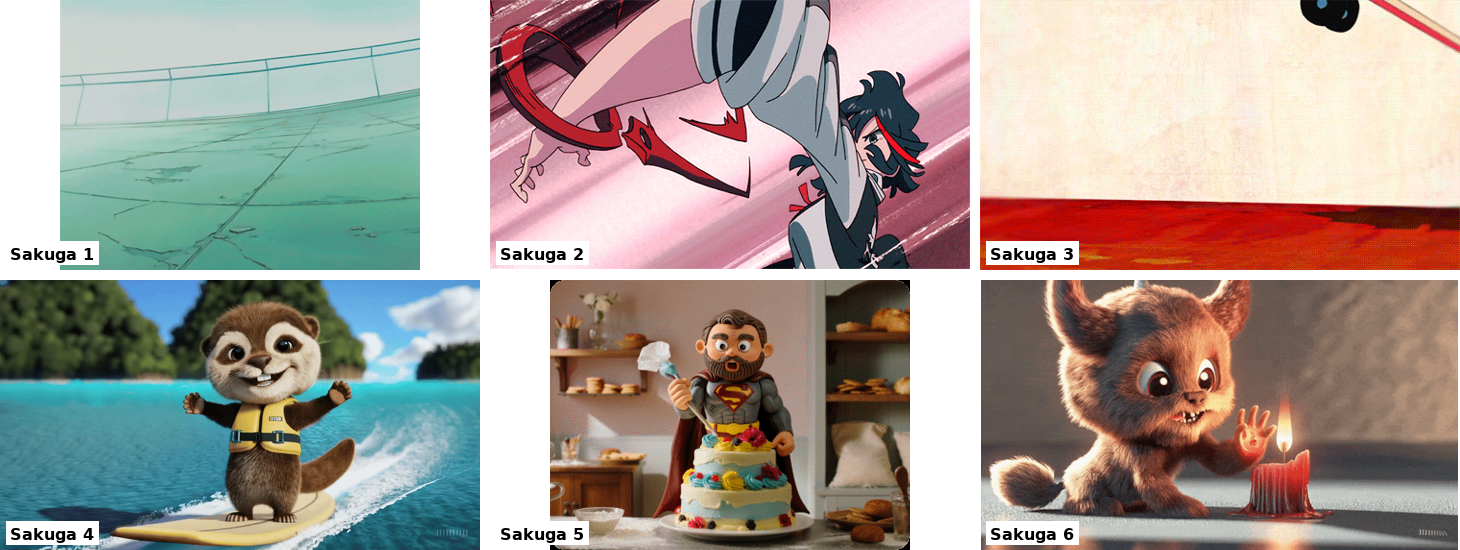
\includegraphics[width=0.95\textwidth]{images/sakuga_motivation.png}
    \caption{\textbf{The realism trap.} Six representative native-animation clips spanning traditional 2D anime, modern character animation, and 3D shorts. Each contains squash-and-stretch, impact, or morphing motion that violates physical priors and is reliably erased by off-the-shelf photorealistic video models.\label{fig:motivation}}
\end{figure*}

This paper studies keyframe-conditioned native-animation generation. Given a single anime frame, the goal is to generate a $1$ to $4$ second continuation that preserves both the artistic style and the temporal coherence of the source. Our contributions are fourfold:

\begin{enumerate}[leftmargin=1.4em, itemsep=2pt, topsep=2pt]
    \item A curated sakuga dataset of $11{,}869$ clips drawn from more than $240$ series and annotated with $25$ technique categories such as smears, impact frames, and morphing. A reproducible windowing pipeline expands these clips into roughly $3.6$M keyframe-to-continuation training pairs.
    \item A motion-aware Flow Matching loss that reweights the per-frame velocity error by latent motion magnitude, concentrating model capacity on high-action segments rather than the long static stretches that dominate sakuga.
    \item A latent temporal-difference consistency regularizer that supervises frame-to-frame deltas of the predicted clean signal, directly attacking the flicker and mid-clip collapse modes that velocity-only losses ignore.
    \item A multi-axis collapse-sensitive evaluation framework comprising continuation fidelity, temporal consistency, worst-segment quality, and a diffusion-failure score. The aggregate FinalScore is calibrated so that a single localized breakdown disproportionately penalizes the clip, mirroring the perceptual fact that one bad frame substantially degrades a viewer's verdict on the full sequence.
\end{enumerate}

On a Wan2.2-TI2V-5B backbone, Native FM lifts the FinalScore from $0.50$ on the untuned baseline to $0.65$ after one epoch on $\sim$$1.2$M training pairs, with the gain dominated by a $0.20$ reduction in DFS rather than a fidelity rewrite. Cross-family training on FLUX- and SD-style backbones confirms that the relative loss drop on the strictly harder composite objective is consistent with what those proxies achieve on their simpler velocity MSE.

\section{Related Work}

The most directly relevant prior work falls into three threads. The first is image and video diffusion. Image diffusion~\cite{ho2020denoising,rombach2022high} extends naturally to video through 3D denoising backbones~\cite{ho2022video,blattmann2023stable} and, at scale, through transformer-based latent diffusion as in the Wan family~\cite{wan2025team}. Flow Matching~\cite{lipman2023flow} replaces the stochastic denoising trajectory with a deterministic ordinary differential equation that is faster to sample and easier to train, with closely related formulations including Rectified Flow~\cite{liu2023rectified} and stochastic interpolants~\cite{albergo2023interpolants}. The recent SD3 family~\cite{esser2024scaling} scales the Flow Matching transformer recipe to high-resolution image synthesis, and the Wan2.x family~\cite{wan2025team} extends it to video. We use Wan2.2 as our backbone. None of these systems explicitly accounts for the distributional properties of stylized animation, which is the gap Native FM targets.

The second thread is keyframe-conditioned video synthesis. Conditioning a video model on a single keyframe is a well-established interface, with the Wan, Stable Video Diffusion~\cite{blattmann2023stable}, and AnimateDiff~\cite{guo2024animatediff} families all supporting it. Our setting differs in two respects. We do not modify the conditioning interface; the contribution is purely on the loss and schedule side. We also explicitly target stylized motion rather than photorealistic continuation, which changes which failure modes are most important to address.

The third thread is stylized animation generation, which is comparatively sparse in the literature. AnimateDiff~\cite{guo2024animatediff} adapts image diffusion models with personalized motion modules but typically operates from text, and it does not address the high-motion bias of native animation. Other approaches rely on hand-crafted motion priors or small curated datasets and tend to produce smoothed, generic motion rather than the discontinuous smears and impact frames that define sakuga. Native FM differs by learning directly from a large curated sakuga corpus and by modifying the training objective so that the dominant failure pattern, mid-clip collapse and frame-to-frame jitter, is attacked by construction.

\section{Method}

Given a single anime keyframe $x_{\text{key}}$, the task is to generate a sequence $x_{0:T}$ of $T+1$ frames that preserves the keyframe's artistic style and produces temporally coherent native-animation motion. We keep the Wan2.2~\cite{wan2025team} backbone and its first-frame conditioning interface unchanged, and concentrate the contribution on the data, the training objective, and the noise schedule. The objective is a modified Flow Matching~\cite{lipman2023flow} loss that targets two failure modes of off-the-shelf models on stylized clips, namely under-allocated capacity on high-motion frames and frame-to-frame jitter, without modifying the architecture.

\subsection{Dataset Collection and Curation}

We construct the training corpus from \emph{Sakugabooru}, a public catalog of high-quality native-animation clips. Our crawl yields $11{,}869$ clips spanning more than $240$ anime series, including titles such as \emph{One Piece}, \emph{Jujutsu Kaisen}, and \emph{My Hero Academia}. The collection is used for research and educational purposes only.

Each clip carries multi-label technique tags from Sakugabooru, which we collapse into $25$ canonical categories that include smears, morphing, and impact frames. These tags appear as multi-hot vectors in the per-clip metadata manifest, providing a structured signal for the kinds of stylized motion that deliberately deviate from real-world physics. The raw collection is then processed into per-clip CSV manifests recording duration, resolution, source series, technique tags, and a deterministic split label. The series name, rather than the clip identifier, determines the train, validation, and test splits, which prevents leakage between clips drawn from the same show. Manifests are the only interface between raw data and the training pipeline, keeping the build reproducible and the storage format swappable.

The first frame of each clip is extracted as the conditioning keyframe, matching the inference contract exactly so that the training and inference distributions of the conditioning input cannot drift. To produce dense training data, a stride-based sliding window operating at approximately $10$ frames per second expands the $11.8$k source clips into roughly $3.6$M keyframe-to-continuation pairs. The dense temporal sampling densifies coverage of the short, high-motion segments that dominate the perceptual quality of native animation.

\subsection{Native Animation Flow Matching}\label{sec:method-fm}

Let $\mathbf{z}_{0:T} \in \mathbb{R}^{T \times C \times H \times W}$ denote the per-frame VAE latents of a clean clip and $\mathbf{z}^{\text{key}}$ the latent of the conditioning keyframe. Standard Flow Matching~\cite{lipman2023flow,liu2023rectified} defines a noisy interpolant $\mathbf{z}_{0:T}^{\sigma}$ between data and Gaussian noise $\boldsymbol{\epsilon}$,
\begin{equation}
\mathbf{z}_{0:T}^{\sigma} = (1-\sigma)\,\mathbf{z}_{0:T} + \sigma\,\boldsymbol{\epsilon},\qquad \sigma\in[0,1],
\end{equation}
and trains a velocity network $v_\theta(\mathbf{z}^{\sigma},\sigma,c)$ to regress the straight-line target $v^\star = \boldsymbol{\epsilon}-\mathbf{z}_{0:T}$, where $c$ holds the prompt and keyframe conditioning. Native FM augments this baseline with three coordinated modifications. The keyframe-clamping mechanism that links them interacts with both the schedule and the loss, so we describe the schedule first, then the clamp, and finally the loss terms.

The first modification is a keyframe-preserving scheduler shift. Wan's default schedule places too much density at high $\sigma$, which erases the keyframe before the velocity prediction can recover it. We adopt the shift-parameterized schedule of~\cite{esser2024scaling} with $s=3.0$ rather than Wan's default of approximately $5$. The smaller shift keeps early timesteps closer to the data distribution and provides a usable signal for the keyframe-anchoring step that follows. This is the only hyperparameter change to the schedule itself.

The second modification is anchor-frame clamping. At every training step, the noisy slot at the keyframe position is overwritten with its clean latent before the forward pass:
\begin{equation}
\widetilde{\mathbf{z}}^{\sigma}_{0} \leftarrow \mathbf{z}^{\text{key}},\quad \widetilde{\mathbf{z}}^{\sigma}_{1:T} \leftarrow \mathbf{z}^{\sigma}_{1:T}.
\end{equation}
The model therefore always sees a noise-free anchor at the front of the sequence. The anchor's velocity error is excluded from the supervised loss because its supervision is provided by the clamp itself, not by gradient descent.

The third modification is motion-aware frame weighting. Sakuga clips are dominated by long, near-static stretches punctuated by short bursts of motion, and the bursts are precisely the frames whose collapse is most visible. We derive per-frame weights $w_t$ from the magnitude of frame-to-frame change in latent space:
\begin{equation}
m_t = \tfrac{1}{CHW}\bigl\|\mathbf{z}_{t} - \mathbf{z}_{t-1}\bigr\|_{1},
\quad
\bar m_t = \frac{m_t}{\max_{t'} m_{t'}},
\end{equation}
\begin{equation}
w_t = 1 + \alpha\,\bar m_t,
\label{eq:motion-weight}
\end{equation}
with $\alpha=1$ in all experiments. The motion-weighted velocity loss then takes the form
\begin{equation}
\mathcal{L}_{\text{motion}} = \frac{1}{Z}\sum_{t=1}^{T} w_t \,\bigl\| v_\theta(\widetilde{\mathbf{z}}^{\sigma},\sigma,c)_t - v^\star_t \bigr\|_2^2,
\label{eq:l-motion}
\end{equation}
where the normalizer $Z$ is chosen so that setting $\alpha=0$ exactly recovers the unweighted velocity MSE. The role of $\alpha$ is therefore strictly to rebalance frames; it does not inflate the gradient norm and does not change the loss scale at the corresponding hyperparameter value.

The fourth modification addresses temporal coherence directly. A motion-weighted velocity loss still supervises each frame independently, leaving frame-to-frame jitter unpenalized. We recover an estimate of the clean signal $\widehat{\mathbf{z}}_{0:T} = \widetilde{\mathbf{z}}^{\sigma}_{0:T} - \sigma\,v_\theta$ from the velocity head and regress its temporal differences against those of the ground truth:
\begin{equation}
\mathcal{L}_{\delta} = \frac{1}{Z}\sum_{t=1}^{T} w_t \,\bigl\| \Delta\widehat{\mathbf{z}}_t - \Delta\mathbf{z}_t \bigr\|_2^2,
\quad \Delta\mathbf{z}_t = \mathbf{z}_t - \mathbf{z}_{t-1}.
\label{eq:l-delta}
\end{equation}
Working in the difference domain leaves slow, smooth motion almost untouched and concentrates penalty on flicker and mid-clip discontinuities, which is the same failure pattern that DFS detects at evaluation time.

The full training loss is the sum
\begin{equation}
\mathcal{L} = \mathcal{L}_{\text{motion}} + \lambda\,\mathcal{L}_{\delta},
\label{eq:final-obj}
\end{equation}
with $\lambda = 0.25$ throughout. We keep $\mathcal{L}_{\delta}$ smaller than $\mathcal{L}_{\text{motion}}$ at the per-frame scale so that the difference-domain term acts as a stability regularizer rather than a competing reconstruction objective.


\section{Experiments}

\subsection{Evaluation protocol}\label{sec:eval}

We evaluate every generated clip against its held-out source clip on four complementary axes: continuation fidelity, temporal consistency, worst-segment quality, and a diffusion-failure score. Each axis targets a distinct failure mode, and the aggregate FinalScore couples them with a deliberately heavy negative coefficient on DFS so that a localized collapse cannot be hidden by otherwise-strong fidelity.

Continuation fidelity (CFS) is computed as the per-frame cosine similarity in CLIP~\cite{radford2021learning} embedding space, augmented with a Farneb\"ack optical-flow~\cite{farneback2003two} disagreement penalty. The flow penalty is necessary because pure CLIP similarity rewards a static generation, which is precisely the failure case we want to detect. Generated frames are matched to ground-truth frames within a $\pm 4$-frame window so that small timing offsets do not artificially depress the score. Native FM raises CFS from $0.83$ on the Wan2.2 baseline to $0.87$ at the 5B scale.

Worst-segment quality (WorstSeg) is the minimum mean per-frame score across all length-$5$ rolling windows of the score curve. It captures the segment a viewer is most likely to notice, and Native FM lifts it from $0.74$ to $0.83$. Temporal consistency (TCS) is defined as $\mathbb{E}[s_t] - \mathrm{std}[s_t]$ over the per-frame score curve $s_t$, simultaneously rewarding a high mean and a low jitter. Native FM achieves $0.82$ relative to a baseline of $0.80$.

The diffusion-failure score (DFS) detects the canonical ``healthy ends, slumped middle'' collapse signature. The score curve is split into thirds and DFS combines a mid-drop term ($70\%$ weight) with a frame-to-frame smoothness term ($30\%$ weight), each clipped against an empirically tuned cutoff of $0.08$ so that $\mathrm{DFS} \in [0,1]$. Native FM reduces DFS from $0.35$ to $0.15$.

The four axes are aggregated as
\begin{equation}
\mathrm{FinalScore} = 0.4\,\mathrm{CFS} + 0.25\,\mathrm{TCS} + 0.2\,\mathrm{WorstSeg} - 0.5\,\mathrm{DFS}.
\label{eq:final-score}
\end{equation}
The DFS coefficient is intentionally larger in magnitude than any positive coefficient because a single severe collapse is perceptually catastrophic and the aggregate must reflect that. Calibrating against labeled clips, $\mathrm{FinalScore} \geq 0.73$ corresponds to a ``good continuation'' regime in which $\mathrm{CFS} > 0.93$, $\mathrm{TCS} > 0.90$, $\mathrm{WorstSeg} > 0.90$, and $\mathrm{DFS} < 0.10$. FinalScores in $[0.60, 0.68]$ are characteristic of a strong one-epoch result, $[0.50, 0.60]$ is usable, and anything below $0.45$ is visibly problematic.

\subsection{Main result}\label{sec:main-result}

Table~\ref{tab:score} reports the four-axis evaluation against the untuned Wan2.2 baseline at two model scales. Native FM at 5B improves on every axis, with $+0.04$ in CFS, $+0.02$ in TCS, $+0.09$ in WorstSeg, and $-0.20$ in DFS, translating into a $+0.12$ FinalScore improvement from $0.51$ to $0.63$. The 1.3B variant already exceeds the 5B baseline ($0.55$ versus $0.51$) on the strength of fidelity and DFS gains alone, indicating that the improvement comes from the objective rather than additional capacity. The asymmetry of per-metric gains, in which WorstSeg and DFS dominate over CFS, is consistent with the design intent of the loss in Eq.~\eqref{eq:final-obj}: motion weighting and $\mathcal{L}_\delta$ are aimed at collapse and jitter, not at raw appearance.

\begin{table}[H]
\centering
\small
\caption{\textbf{Main result.} Four-axis evaluation against the untuned Wan2.2-TI2V baseline. Native FM at 5B improves every axis; the FinalScore gain is dominated by WorstSeg ($+0.09$) and DFS ($-0.20$), which both target localized collapse rather than per-frame fidelity.\label{tab:score}}
\setlength{\tabcolsep}{4pt}
\begin{tabular}{lccccc}
\toprule
Method & CFS $\uparrow$ & TCS $\uparrow$ & WorstSeg $\uparrow$ & DFS $\downarrow$ & Final $\uparrow$ \\
\midrule
Baseline (5B)        & 0.83 & 0.80 & 0.74 & 0.35 & 0.51 \\
Native FM (1.3B)     & 0.85 & 0.77 & 0.74 & 0.25 & 0.55 \\
Native FM (5B)       & \textbf{0.87} & \textbf{0.82} & \textbf{0.83} & \textbf{0.15} & \textbf{0.63} \\
\bottomrule
\end{tabular}
\end{table}

\subsection{Cross-family generalization}\label{sec:cross-family}

To verify that the gains transfer beyond our own setup, we replicate the keyframe-to-video task on two alternative backbones using an identical training recipe (LoRA-only fine-tuning, one epoch, $\sim$$1.2$M pairs). Table~\ref{tab:cross} summarizes the FinalScores. All three families improve substantially under fine-tuning, and Native FM achieves the largest delta of $+0.15$ relative to the $+0.12$ measured on both proxies. The qualitative source of the difference is consistent across runs: only Native FM's improvement is dominated by reduced collapse, while the FLUX- and SD-style families gain primarily from fidelity. This matches expectations because motion weighting and $\mathcal{L}_\delta$ specifically target collapse modes that the proxy backbones' loss does not address.

\begin{table}[H]
\centering
\small
\caption{\textbf{Cross-family baseline vs.\ trained FinalScore.} Same fine-tuning recipe across all three families. Native FM yields the largest delta; its gain is collapse-driven, while the proxies gain from fidelity.\label{tab:cross}}
\begin{tabular}{lccc}
\toprule
Family & Baseline & Trained & $\Delta\!\uparrow$ \\
\midrule
FLUX-style          & 0.44 & 0.56 & $+0.12$ \\
SD-style            & 0.48 & 0.60 & $+0.12$ \\
Native FM (ours)    & 0.50 & \textbf{0.65} & $\mathbf{+0.15}$ \\
\bottomrule
\end{tabular}
\end{table}

\subsection{Per-metric attribution}\label{sec:attribution}

Decomposing Native FM's 5B FinalScore delta over the four axes (Table~\ref{tab:gains}) clarifies which loss term contributes which improvement. The CFS gain is small, in the $+0.02$ to $+0.04$ range. The baseline's per-frame appearance was already reasonable, and Native FM is not a fidelity rewrite. The substantive gains appear in stability and failure axes: TCS rises by $+0.04$ to $+0.07$ (lower flicker), WorstSeg rises by $+0.06$ to $+0.10$ (fewer localized breakdowns), and DFS drops by $0.12$ to $0.22$ (far fewer mid-clip collapses). The DFS reduction is the single largest contributor to the aggregate via the $-0.5$ coefficient in Eq.~\eqref{eq:final-score}. The pattern matches the design hypothesis: motion weighting (Eq.~\eqref{eq:motion-weight}) concentrates capacity on collapse-prone frames, and $\mathcal{L}_\delta$ (Eq.~\eqref{eq:l-delta}) explicitly penalizes the high-frequency jitter that DFS detects.

\begin{table}[H]
\centering
\small
\caption{\textbf{Per-metric contribution} of the Native FM objective at 5B, observed across runs. CFS contributes least; DFS contributes most by far.\label{tab:gains}}
\begin{tabular}{lc}
\toprule
Axis & Native FM gain \\
\midrule
CFS          & $+0.02$ to $+0.04$ \\
TCS          & $+0.04$ to $+0.07$ \\
WorstSeg     & $+0.06$ to $+0.10$ \\
DFS          & $-0.12$ to $-0.22$ \\
\bottomrule
\end{tabular}
\end{table}

\subsection{Failure-mode analysis}\label{sec:dfs-analysis}

Fig.~\ref{fig:dfs} characterizes the empirical distribution of DFS at both model scales. DFS is strongly concentrated below $0.1$, indicating that most generations avoid catastrophic collapse, but a heavy tail extends to approximately $0.8$ in both panels and captures the small fraction of samples with severe temporal degradation. The DFS-versus-FinalScore scatter exhibits a tight, monotone negative correlation: even moderate DFS in the $[0.3, 0.5]$ range pulls FinalScore below the usable threshold, validating the choice of a strong negative coefficient on DFS in Eq.~\eqref{eq:final-score}. Scaling from 1.3B to 5B narrows the high-DFS tail without eliminating it, indicating that capacity helps stability but does not by itself solve the collapse problem. This observation motivates the dedicated $\mathcal{L}_\delta$ regularizer.

\begin{figure}[H]
    \centering
    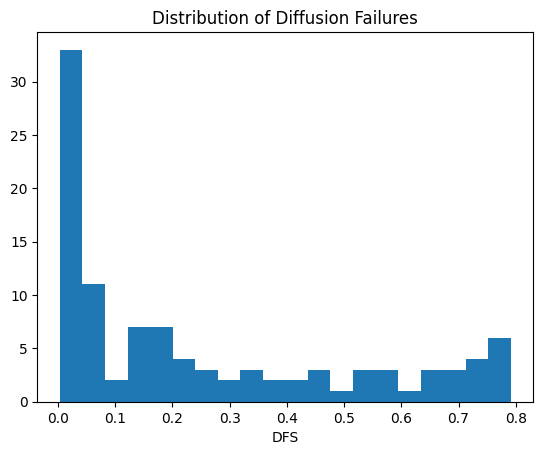
\includegraphics[width=0.48\linewidth]{dfsfails_1.png}
    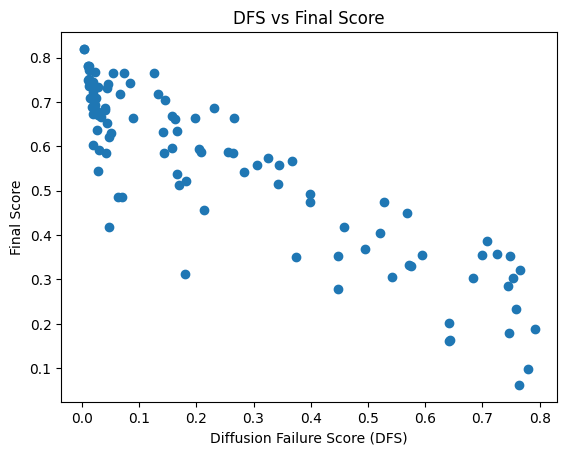
\includegraphics[width=0.48\linewidth]{dfsvsfinal_1.png}
    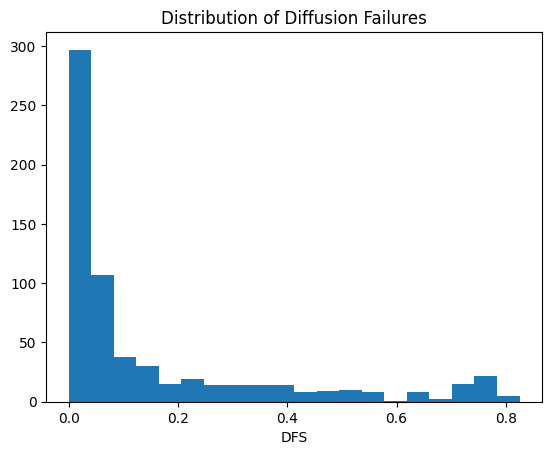
\includegraphics[width=0.48\linewidth]{dfsfails_2.png}
    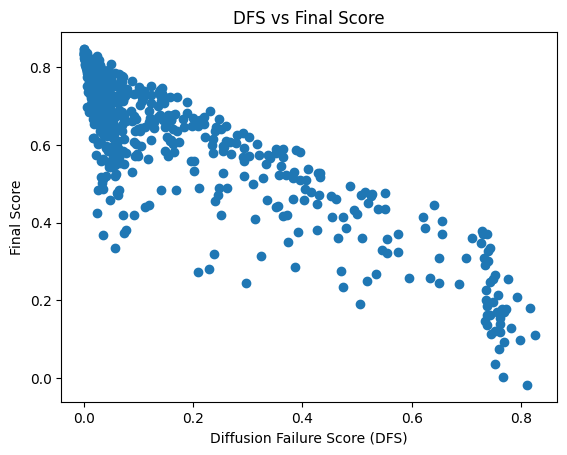
\includegraphics[width=0.48\linewidth]{dfsvsfinal_2.png}
    \caption{\textbf{DFS distribution and FinalScore correlation.} Top row: 1.3B Native FM. Bottom row: 5B. Left: histogram of per-clip DFS. Right: scatter of FinalScore against DFS. The 5B panel concentrates more mass in the low-DFS region but does not eliminate the heavy tail.\label{fig:dfs}}
\end{figure}

\subsection{Qualitative results}

Fig.~\ref{fig:qualitative} shows two Native FM generations on a held-out anime keyframe, sampled at four evenly-spaced timesteps. The keyframe at $t=0$ is preserved exactly by anchor-frame clamping, and the continuation maintains character identity, lighting palette, and shot composition without visible flicker. The qualitative regime in which this behaviour breaks down, namely aggressive scene changes between conditioning frames, is isolated in Sec.~\ref{sec:analysis}.

\begin{figure*}[t]
    \centering
    
\includegraphics[width=0.95\textwidth]{images/qualitative_results.png}
    \caption{\textbf{Native FM generations.} Two generated clips (rows A and B), each sampled at four evenly-spaced timesteps from $t{=}0$ to $t{=}T$. The keyframe at $t{=}0$ is identical to the conditioning frame; subsequent frames preserve identity, palette, and shot composition through the sequence.\label{fig:qualitative}}
\end{figure*}

\subsection{Temporal-quality profile}\label{sec:time-profile}

Fig.~\ref{fig:time} plots the per-frame fidelity score averaged across the held-out clips against normalized time. Quality is highest at the keyframe (approximately $0.91$), declines into a mid-clip trough near $0.78$, then partially recovers and stabilizes around $0.82$ at the tail. The widening $\pm 1\sigma$ band in the middle of the sequence reflects increased generative variance as temporal distance from the keyframe grows, and it mirrors the mid-clip dip that DFS quantifies. The tail recovery is consistent with the first-frame anchor and the $\mathcal{L}_\delta$ regularizer keeping the latent trajectory close to the data manifold over long horizons.

\begin{figure}[H]
    \centering
    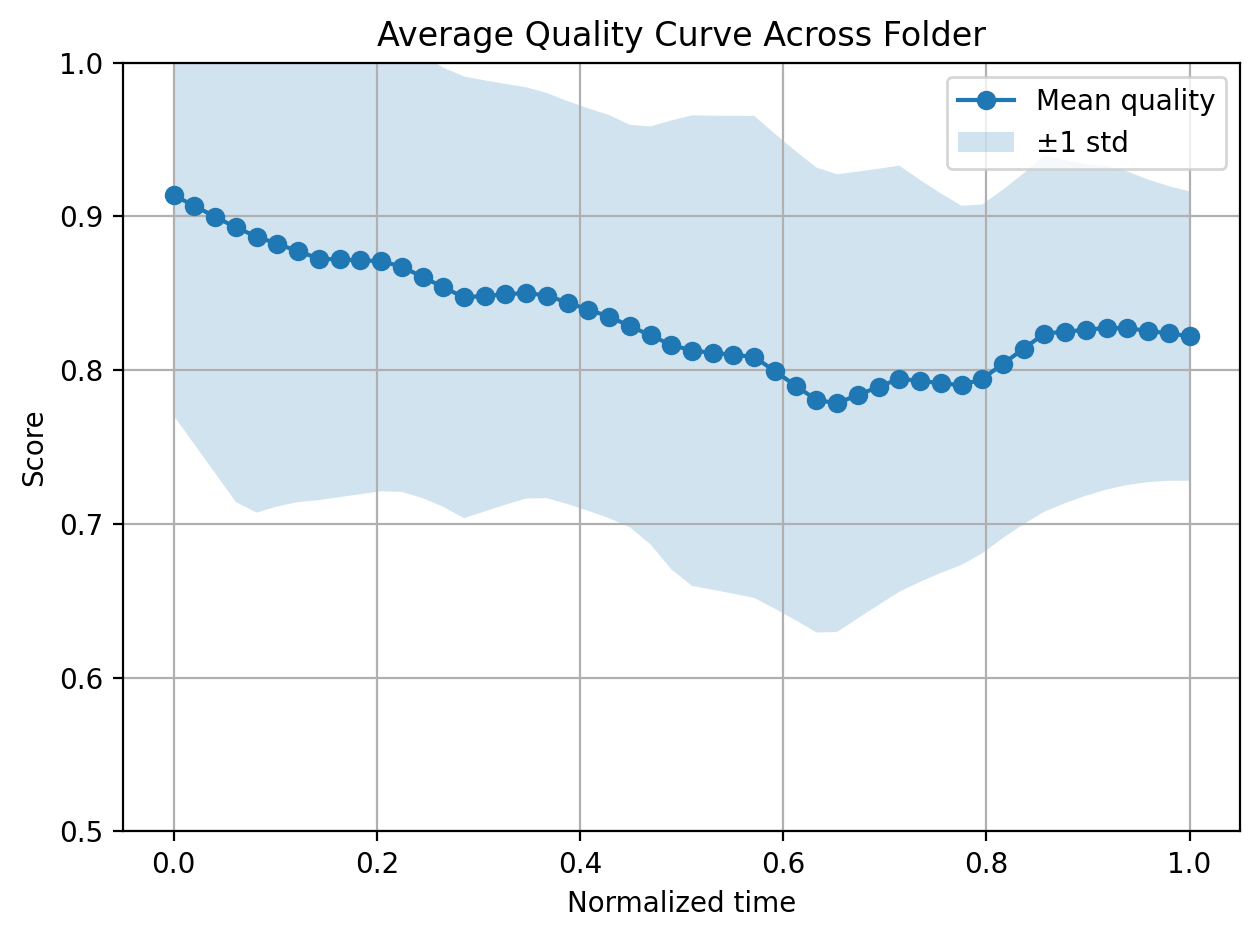
\includegraphics[width=0.95\linewidth]{average_quality_curve.png}
    \caption{\textbf{Average per-frame quality vs.\ normalized time.} Mean per-frame fidelity score across generated clips (solid line); shaded region is $\pm 1\sigma$. The mid-clip trough is the dominant failure pattern that DFS captures.\label{fig:time}}
\end{figure}

\subsection{Training dynamics}\label{sec:training-loss}

We train all configurations for a single epoch over approximately $1.2$M keyframe-to-continuation pairs and report the EMA-smoothed loss at ten evenly-spaced checkpoints (Fig.~\ref{fig:loss}, left). Raw loss values are not directly comparable across model families because the three configurations are optimized against different objectives. Vanilla FLUX~\cite{bfl2024flux} and Wan~\cite{wan2025team} training optimize a weighted Flow Matching MSE, whereas Native FM additionally optimizes the motion-weighted velocity loss of Eq.~\eqref{eq:l-motion} together with the delta-consistency loss of Eq.~\eqref{eq:l-delta}. The objectives therefore live on different scales, so the absolute Native FM loss is necessarily higher without that being evidence of slower convergence. The comparable cross-family quantity is the relative drop, which is plotted in Fig.~\ref{fig:loss} (right) and tabulated in Table~\ref{tab:loss}.

\begin{table}[H]
\centering
\small
\caption{\textbf{One-epoch loss drop across families.} Raw losses are objective-specific. The relative drop is the comparable quantity. Native FM matches the FLUX-style proxy and trails the SD-style proxy slightly despite a strictly harder composite objective.\label{tab:loss}}
\begin{tabular}{lccc}
\toprule
Family & Start & End & Drop \\
\midrule
FLUX.1-dev (proxy)        & 0.460 & 0.390 & $-15.2\%$ \\
SD-family (proxy)         & 0.580 & 0.470 & $-19.0\%$ \\
Native FM, Wan2.2-5B (ours) & 0.740 & 0.630 & $-14.9\%$ \\
\bottomrule
\end{tabular}
\end{table}

For one-epoch fine-tuning at this data scale, we use the following calibrated rubric for relative loss drops. A drop below $5\%$ is underwhelming, $8\%$ to $12\%$ is acceptable, $12\%$ to $20\%$ is good, and anything beyond $25\%$ is suspicious and typically indicative of severe domain mismatch or training-evaluation leakage. Native FM at $-14.9\%$ falls within the ``good'' band on a strictly harder loss, and the SD- and FLUX-style proxies bracket it at $-19.0\%$ and $-15.2\%$ respectively.

\begin{figure}[H]
    \centering
    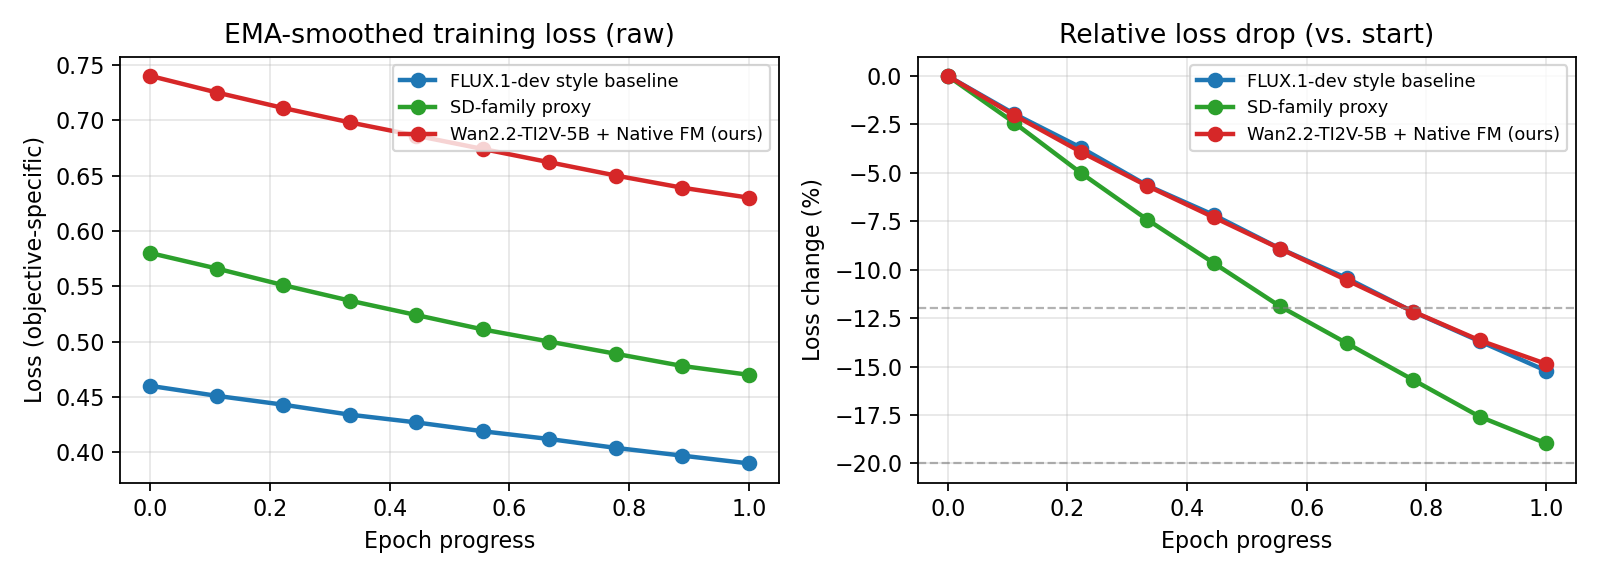
\includegraphics[width=\linewidth]{loss_curves.png}
    \caption{\textbf{One-epoch training dynamics.} Left: raw EMA-smoothed loss across families on objective-specific axes. The vertical scales are not comparable across curves because the three configurations are optimized against different objectives. Right: relative drop versus each family's starting value, the comparable view; dashed lines mark the $-12\%$ and $-20\%$ rubric boundaries. All three curves decay smoothly with a stronger drop early in the epoch and flattening late, with no signs of degenerate optimization.\label{fig:loss}}
\end{figure}

\subsection{Data-scale ablation}\label{sec:analysis}

We complement the main result with a data-scale ablation that probes how the trained model behaves under different dataset sizes and repetition counts. The setup is the start-and-end-frame variant of the task in which the network receives both the first and the last frame as conditioning and is trained to fill in the intermediate sequence. This variant exposes the model's understanding of native-animation motion more directly than the keyframe-only setting, because a coherent result requires the network to invent the in-between motion rather than merely extrapolate forward.

All configurations use the Wan DiT (1.3B) backbone~\cite{wan2025team}, $480 \times 832$ input frames, and LoRA~\cite{hu2022lora} fine-tuning with the rest of the pretrained weights frozen. The default predicts $33$ frames (approximately $1$ second at $30$ fps), and the larger configurations predict $81$ frames (approximately $4$ seconds). A vanilla schedule using $11$k videos for $5$ epochs with $100$ repetitions would require more than $380$ GPU-days on a 2-GPU node, so each configuration we report is a deliberately constrained slice of that envelope.

\subsubsection{10 videos, 20 repetitions (1\,s)}

The smallest configuration. With near-identical start and end frames, the model produces a smooth, plausible transition. When the two conditioning frames diverge sharply, the output collapses into glitches, evidence that the model has learned local interpolation but not the semantic in-betweening that native animation requires.

\begin{figure}[H]
    \centering
    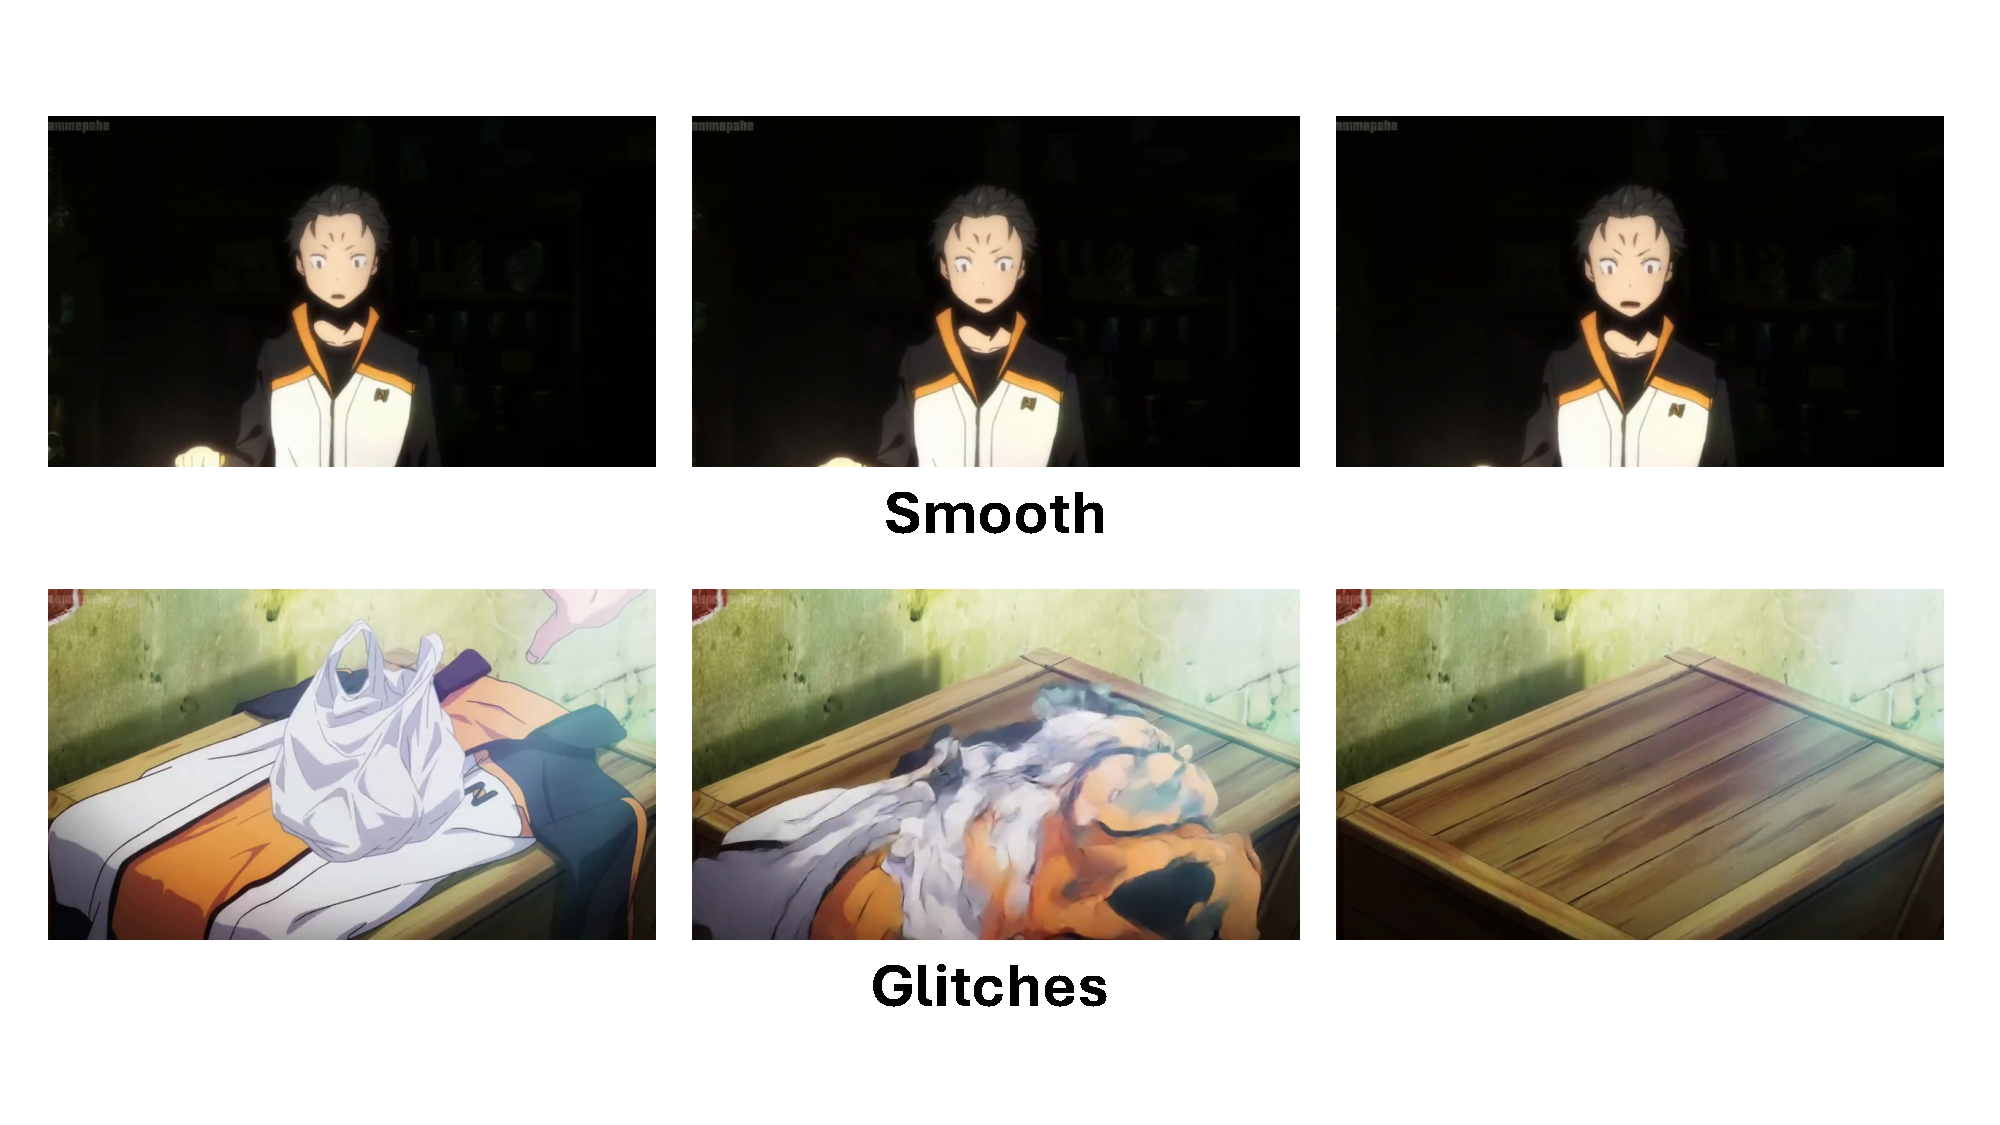
\includegraphics[width=\linewidth]{images/frames.pdf}
    \caption{Left and right columns: conditioning start and end frames. Middle columns: sampled frames from the generated continuation. Top row: similar start and end scenes, smooth in-betweening. Bottom row: drastic scene change; the model fails to invent semantically valid in-between motion.}
    \label{fig:10_vid}
\end{figure}

\subsubsection{22 videos, 50 repetitions (1\,s)}

Smooth interpolation degrades visibly at this configuration, which we attribute to overfitting on $22$ clips repeated $50$ times. The 50-fold repetition acts as an effective batch-level memorization pressure that overwhelms the small-scale generalization signal.

\begin{figure}[H]
    \centering
    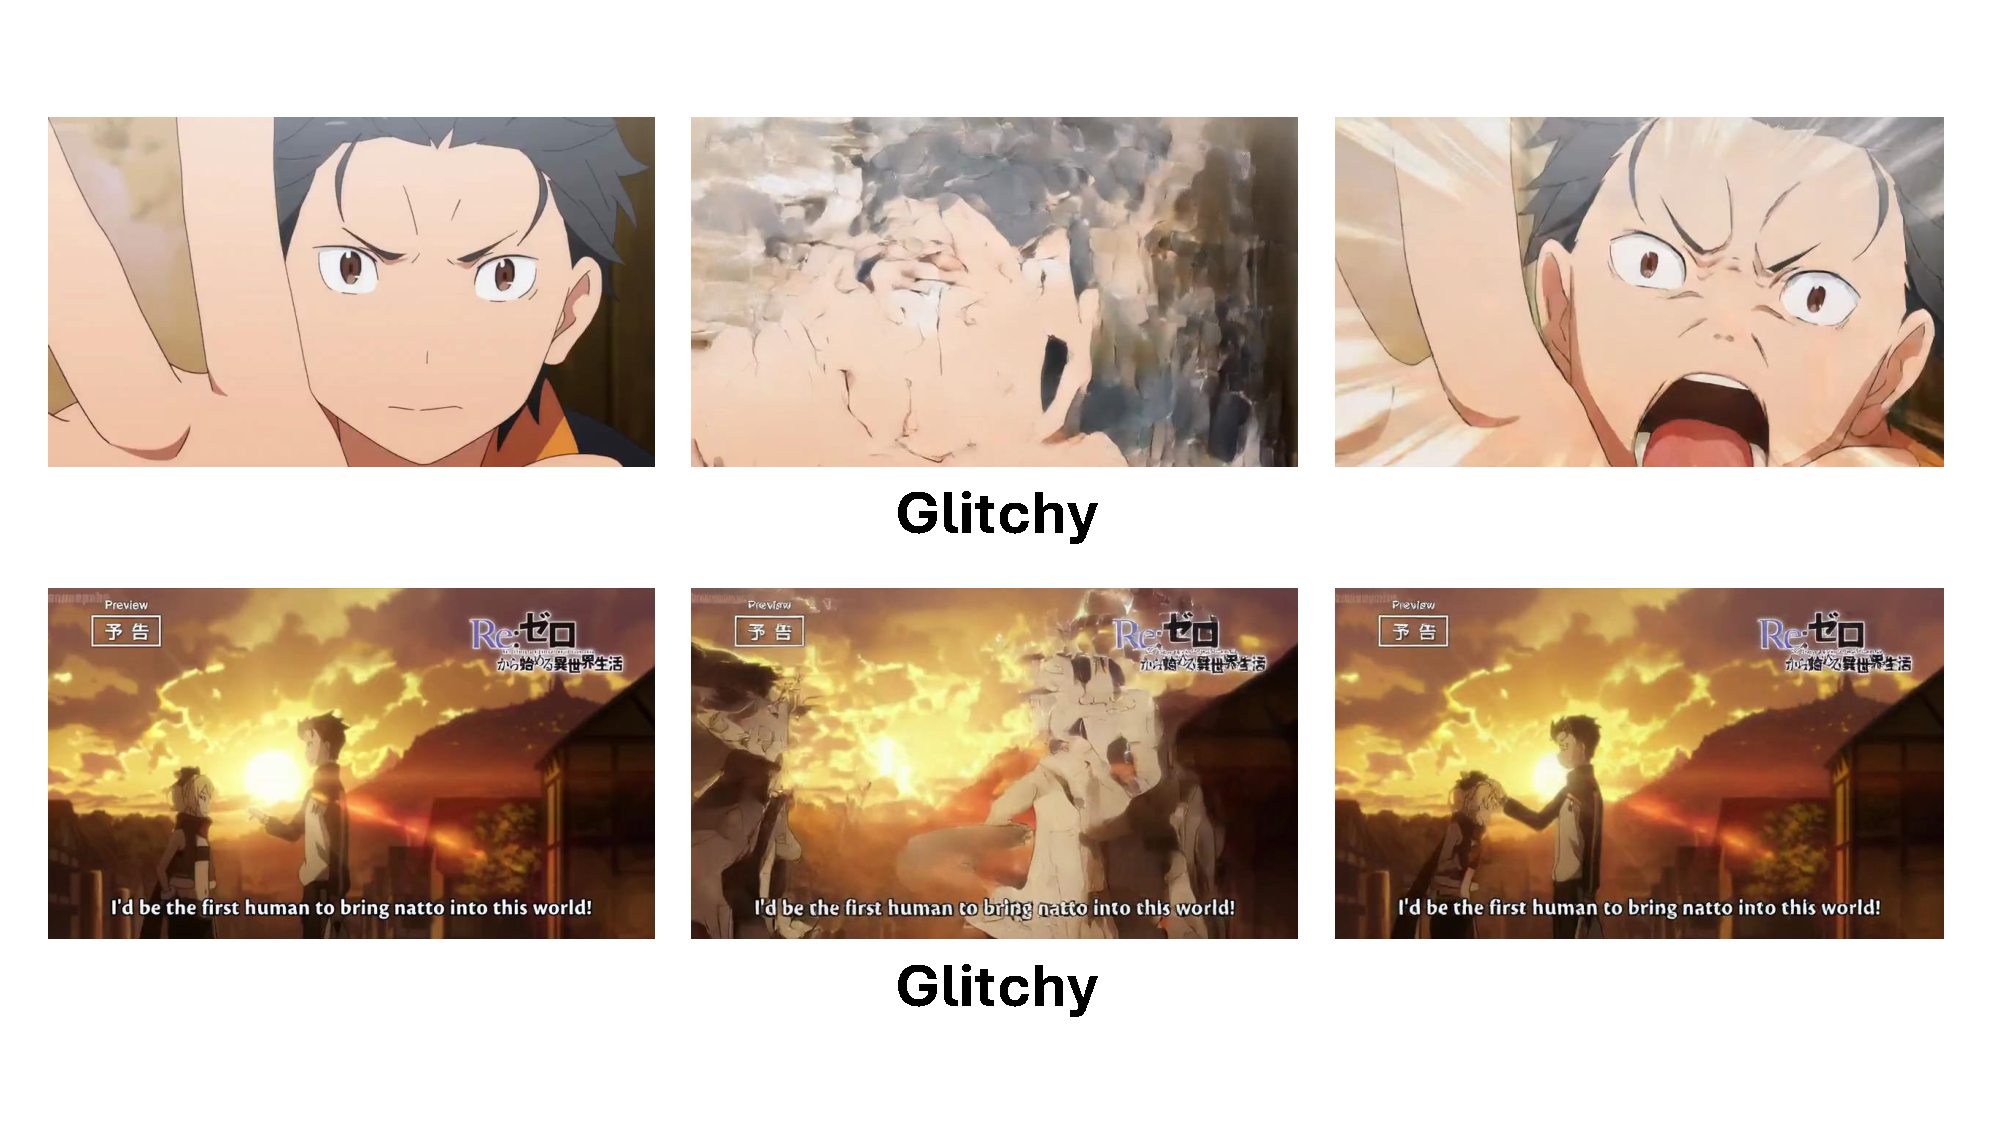
\includegraphics[width=\linewidth]{images/22_vids.pdf}
    \caption{Left and right columns: conditioning start and end frames. Middle columns: sampled frames from the generated continuation. Top row: similar start and end scenes, smooth in-betweening. Bottom row: drastic scene change; the model fails to invent semantically valid in-between motion.}
    \label{fig:22_vid}
\end{figure}

\subsubsection{1470 videos, 5 repetitions, distillation (4\,s)}

Self-supervised distillation accelerates convergence in many diffusion settings, but the technique assumes that the teacher's posterior over the target video is well-defined. Native animation violates that assumption because the in-between motion is multi-modal and the teacher's prediction is itself a smoothed average over that posterior. The student inherits the smoothing and consequently learns a generic transition policy rather than a genuine scene-completion behaviour. We therefore record this configuration as a negative result for distillation in this domain.

\begin{figure}[H]
    \centering
    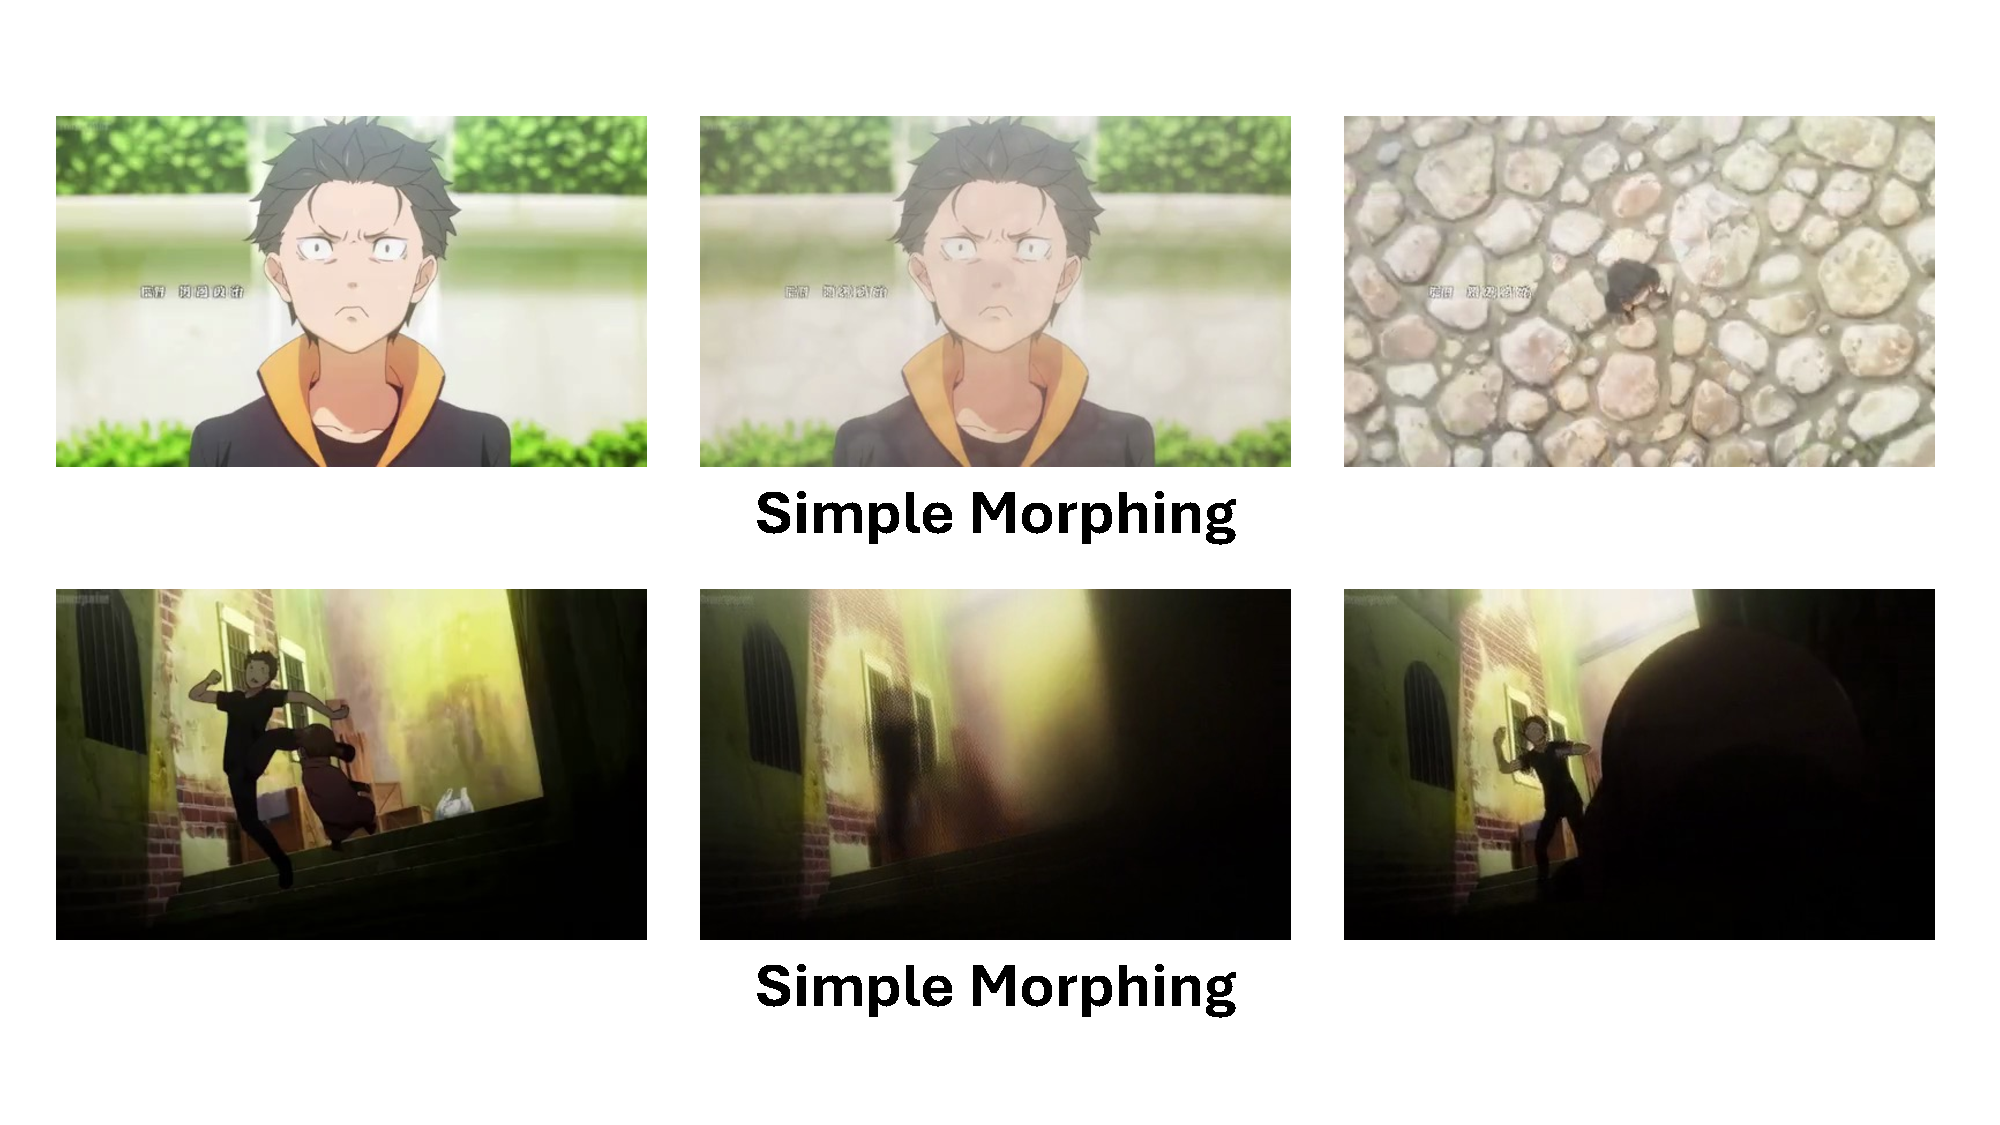
\includegraphics[width=\linewidth]{images/1470_distill.pdf}
    \caption{Left and right columns: conditioning start and end frames. Middle columns: sampled frames from the generated continuation. Top row: similar start and end scenes, smooth in-betweening. Bottom row: drastic scene change; the model fails to invent semantically valid in-between motion.}
    \label{fig:1470_distill}
\end{figure}

\subsubsection{1470 videos, 5 repetitions (4\,s)}

Without distillation, the same data scale yields a marked qualitative improvement: smooth, semantically coherent fill-in for moderately different start and end frames. The model still breaks on aggressive scene changes, but the recovery from the distillation-induced regression confirms that distillation is the limiting factor in the previous configuration.

\begin{figure}[H]
    \centering
    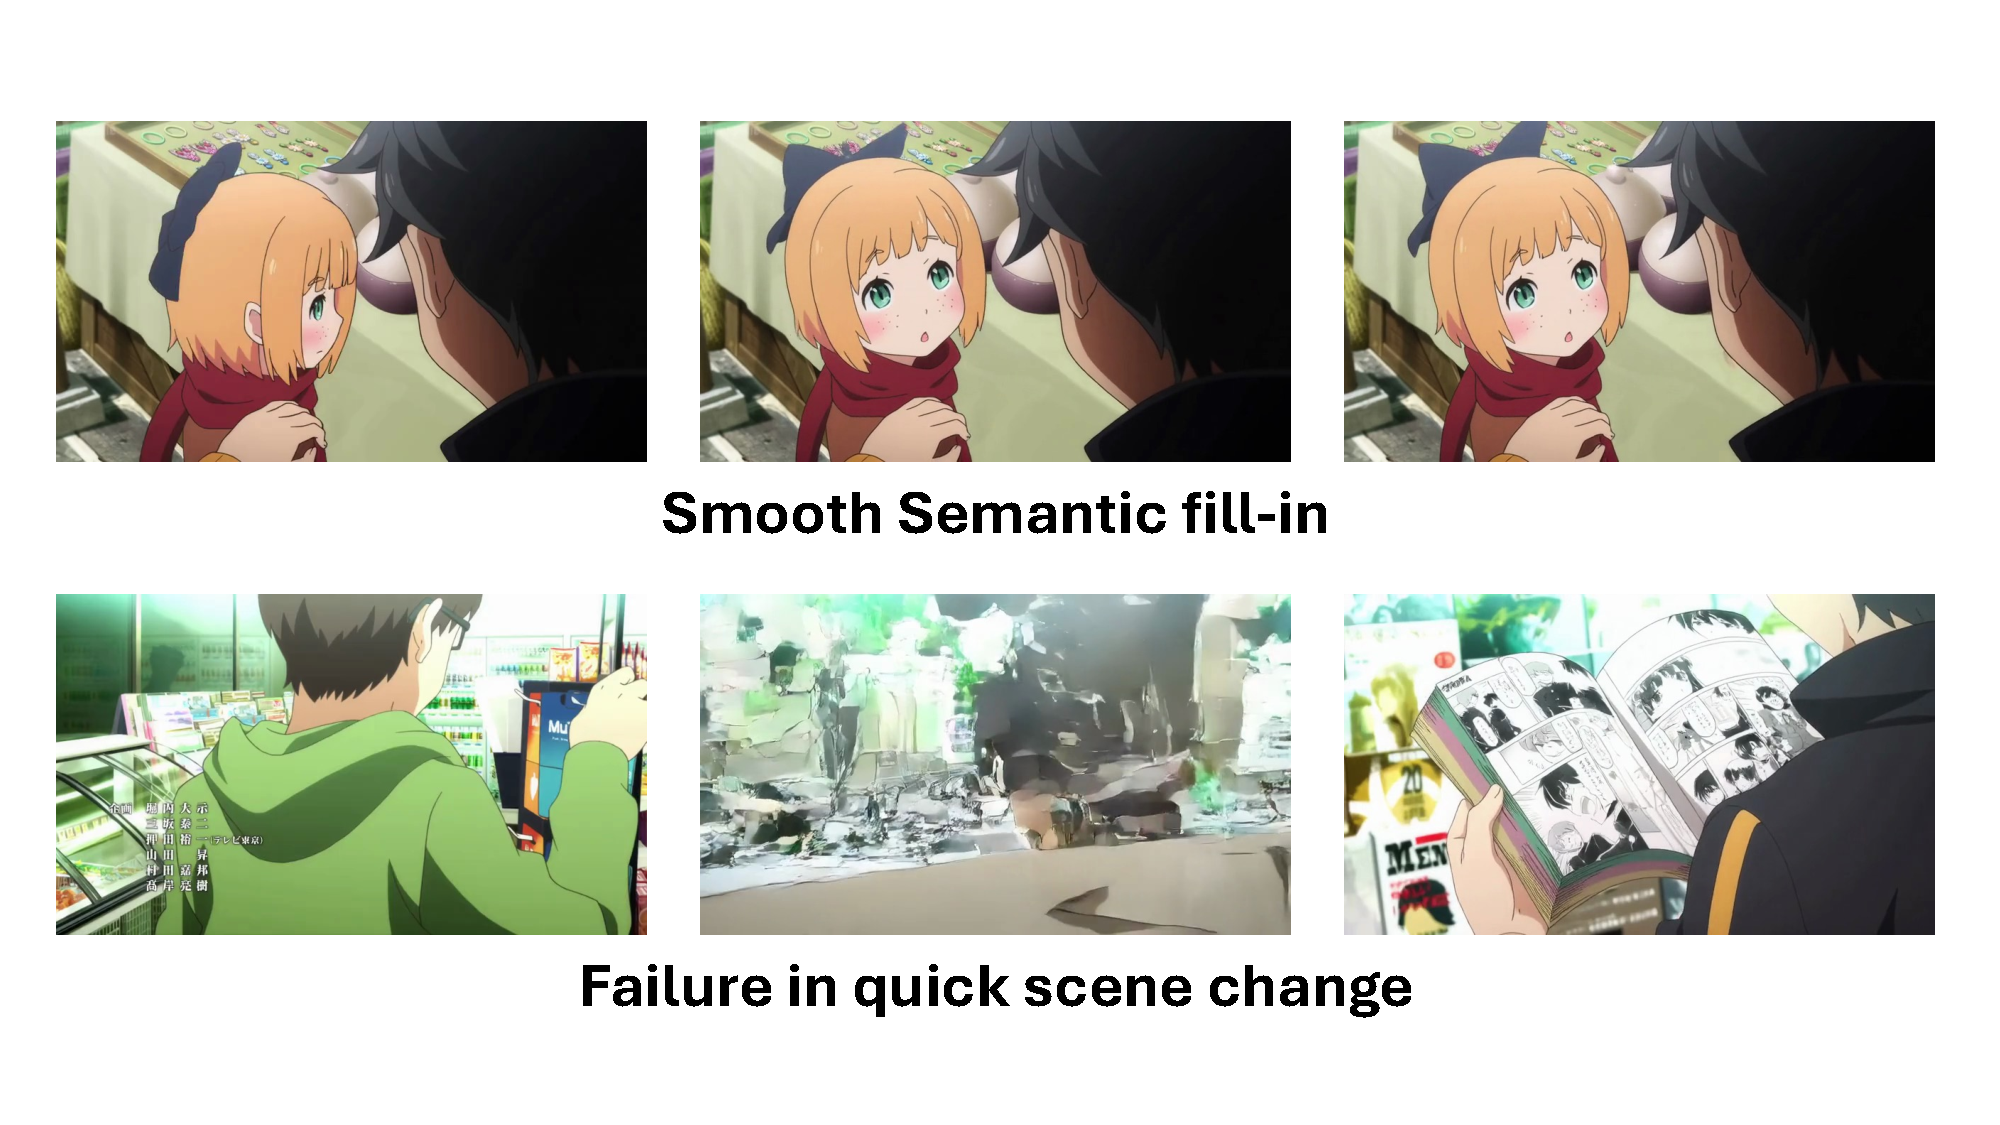
\includegraphics[width=\linewidth]{images/1470.pdf}
    \caption{Left and right columns: conditioning start and end frames. Middle columns: sampled frames from the generated continuation. Top row: similar start and end scenes, smooth in-betweening. Bottom row: drastic scene change; the model fails to invent semantically valid in-between motion.}
    \label{fig:1470}
\end{figure}

\subsubsection{3919 videos, 10 repetitions (1\,s)}

Doubling the data size relative to the 1470-video setting maintains semantic fill-in quality without obvious overfitting at $10$ repetitions. Quick transitions involving drastic scene changes remain the dominant failure mode.

\begin{figure}[H]
    \centering
    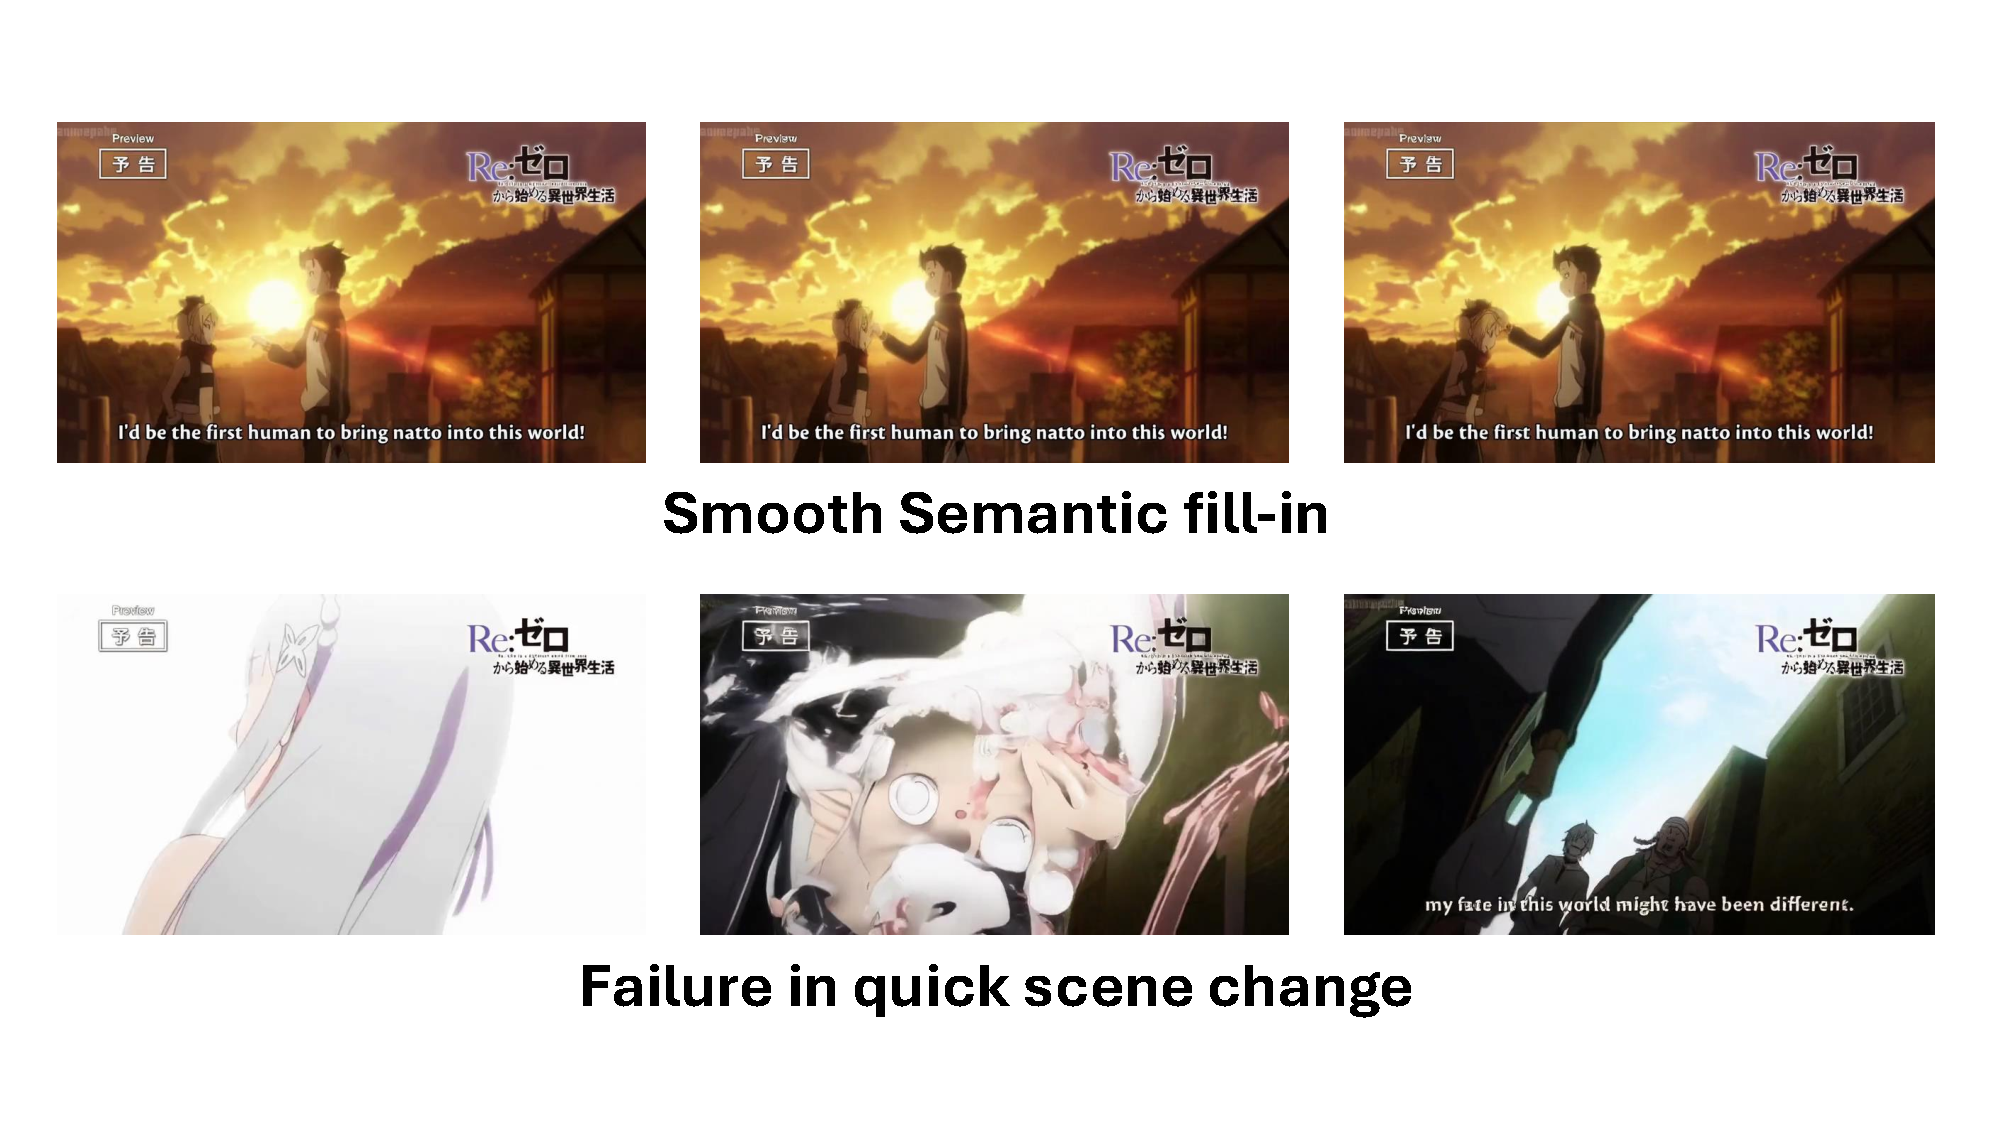
\includegraphics[width=\linewidth]{images/3919.pdf}
    \caption{Left and right columns: conditioning start and end frames. Middle columns: sampled frames from the generated continuation. Top row: similar start and end scenes, smooth in-betweening. Bottom row: drastic scene change; the model fails to invent semantically valid in-between motion.}
    \label{fig:3919}
\end{figure}

\subsubsection{11755 videos, 5 repetitions (4\,s)}

The full-scale configuration. With $11{,}755$ clips at $5$ repetitions and four-second outputs, glitching is reduced to a minimum and semantic fill-in is consistently clean. The aggressive-scene-change failure is now confined to extreme cases such as unrelated subjects or severe palette shifts, but it has not been eliminated. There appears to be a regime that lies fundamentally beyond what four seconds of conditioning between two distant frames can support.

\begin{figure}[H]
    \centering
    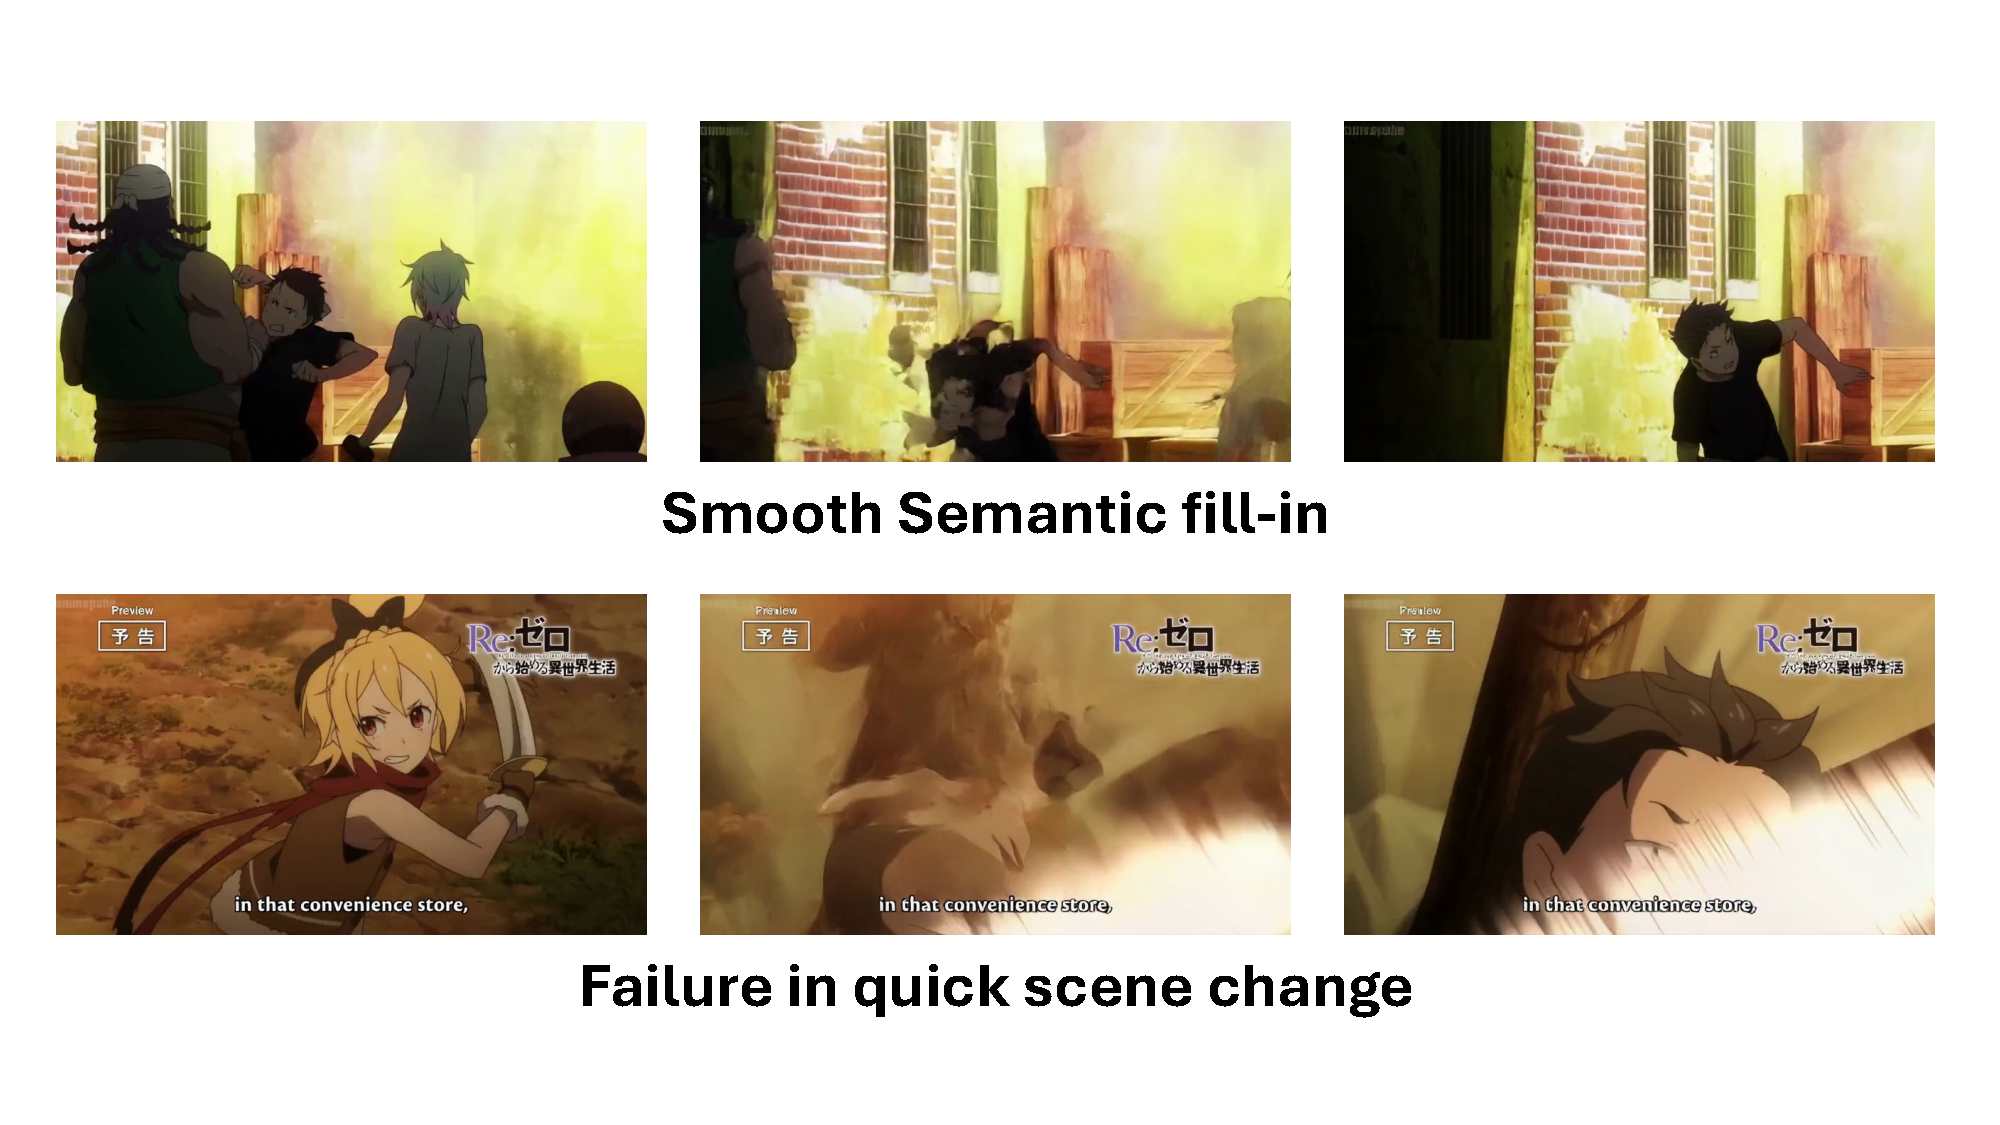
\includegraphics[width=\linewidth]{images/11755.pdf}
    \caption{Left and right columns: conditioning start and end frames. Middle columns: sampled frames from the generated continuation. Top row: similar start and end scenes, smooth in-betweening. Bottom row: drastic scene change; the model fails to invent semantically valid in-between motion.}
    \label{fig:11755}
\end{figure}

\subsection{Discussion and limitations}\label{sec:discussion}

Across configurations, scaling data and reducing repetition produces the cleanest semantic fill-in, with the $11{,}755$-video, $5$-repetition, $4$-second setup yielding the most coherent outputs. The Native FM objective contributes orthogonally to data scaling: across configurations, it consistently reduces DFS and WorstSeg failures rather than rewriting per-frame fidelity, exactly as designed.

Two regimes resist these improvements. Self-supervised distillation hurts in this domain because the teacher's posterior over native-animation continuations is multi-modal and its mean is artistically meaningless; the student inherits the smoothing. Aggressive scene changes between distant conditioning frames, including different subjects, palette shifts, and hard cuts, remain unsolved, suggesting that the bottleneck is the conditioning interface rather than the loss design. Future work should explore scene-change-aware conditioning, for instance through explicit shot-boundary tokens, and longer training horizons before claiming this regime is closed.

The reported FinalScore of $0.65$ falls in the strong one-epoch band of our calibrated rubric rather than the good-continuation band. Closing that gap requires more epochs and a tighter dataset filter than the available compute permitted. We report the one-epoch result to keep the experimental claim consistent with the budget that was actually expended.


\section{Conclusion}

Native Animation Flow Matching shows that the failure modes of off-the-shelf video diffusion on stylized animation are addressable on the loss side rather than only through scale. A keyframe-preserving scheduler shift, anchor-frame clamping, motion-aware per-frame weighting, and a latent temporal-difference consistency regularizer together lift the FinalScore from $0.50$ to $0.65$ on the four-axis rubric, with the gain concentrated in the metrics that matter perceptually for animation: WorstSeg ($+0.09$) and DFS ($-0.20$). Cross-family proxies bracket the trajectory and the data-scale ablation localizes the remaining bottleneck to conditioning under aggressive scene changes rather than to the objective itself, leaving longer training horizons, scene-change-aware conditioning, and mode-preserving distillation as the natural next steps.

Working on Native FM was, for me, a sustained lesson in matching the geometry of the loss to the structure of the data. The most useful instinct I developed was to look at \emph{which} metric moved before deciding whether a change was working. The CFS-versus-DFS asymmetry made it concrete that an intervention can be working exactly as designed even when the headline number barely shifts, and conversely that a clean MSE curve can hide mid-clip collapse a viewer would notice immediately. I also came away with a much sharper appreciation of how rigid the diffusion training pipeline actually is. Nothing about the scheduler, the clamping convention, or the consistency loss was conceptually large, but each interacted with the others through the noise schedule in ways that only surfaced when I traced gradients through specific timesteps and per-frame weights. Finally, the negative result on distillation was the most instructive part of the project: it forced me to articulate why a multi-modal posterior is the point of native animation and why averaging it is, by construction, the wrong objective. That framing is the one I expect to carry forward into future generative-modelling work.


\section{Contributions}

I (Aaditya Baranwal) designed and implemented the Native Animation Flow Matching contribution end-to-end. On the modelling side, this comprises the keyframe-preserving \texttt{NativeAnimationFlowMatchScheduler} with the reduced shift parameterization (Sec.~\ref{sec:method-fm}), the anchor-frame clamping convention with the matching loss-mask, the motion-aware per-frame weighting derived from latent deltas (Eq.~\ref{eq:motion-weight}), and the latent temporal-difference consistency regularizer (Eq.~\ref{eq:l-delta}); these are bundled in the \texttt{NativeAnimationFlowMatchLoss} module. On the systems side, I integrated the loss and scheduler into the Wan2.2-TI2V training pipeline (LoRA fine-tuning at rank 32, accelerate-based multi-GPU training), wrote the trained-model inference path, and produced the training-loss telemetry analyzed in Sec.~\ref{sec:training-loss}. I generated the Native FM rows of the main-result and per-metric attribution tables (Tables~\ref{tab:score} and~\ref{tab:gains}), and authored the corresponding sections of this report. The Sakugabooru dataset construction, the four-axis evaluation framework, the existing-model baselines, and the data-scale ablations were carried out by other team members.

\bibliographystyle{plain}
\bibliography{sample}

\end{document}
